%   %==========================================================================
%   %  Section
%   %==========================================================================
    \section{電場の定義}
    \subsection{クーロンの法則(復習)}
        \begin{mycomment}
            クーロンの法則についての詳細は,\ref{sec:CoulomnbForce}節を参照.
            以下は,そこからの抜粋である.
        \end{mycomment}

            ここに,電荷が2つあるとしよう.この2つの電荷は区別する
            ことができて,$q_{1}$,$q_{2}$ という電気量を持っている
            とする.電荷 $q_{1}$ と $q_{2}$ との距離を $r$ としたと
            き,この2つの電荷が受ける力は,以下のような規則がある.
            \begin{itemize}
                \item 2つの電荷の電気量が互いに異なる符号をもってい
                      るならば,両電荷は互いに引き合う向きに力を受
                      ける
                \item 2つの電荷の電気量が同じ符号を持っているならば,
                      両電荷は互いに反発しあう向きに力を受ける.
                \item 2つの電荷の受ける力の大きさは等しく,
                      向きは互いに逆向きである
                \item 2つの電荷が受ける力の大きさは,
                      2つの電荷の電気量の積($q_{1}q_{2}$)に比例する.
                \item 2つの電荷が受ける力の大きさは,
                      2つの電荷間の距離の2乗($r^{2}$)に反比例する.
            \end{itemize}

        図\ref{fig:coulombs_low}をもう一度載せておこう.
        \begin{figure}[hbt]
            \begin{tabular}{cc}
                \begin{minipage}{0.5\hsize}
                    \begin{center}
                        \includegraphicsdouble{coulombs_low1.pdf}
                    \end{center}
                \end{minipage}
                \begin{minipage}{0.5\hsize}
                    \begin{center}
                        \includegraphicsdouble{coulombs_low2.pdf}
                    \end{center}
                \end{minipage}
            \end{tabular}
        \end{figure}


            次の数式によって,クーロンの法則は表現される.

            電荷 $q_{1}$ に対して働く力は,以下.
               \begin{align}\label{eq:coulomb_force_f1_2nd}
                   \bF_{21} =
                       \frac{1}{4\pi\varepsilon_{0}} \frac{q_{1}q_{2}}{r^{2}}
                           \frac{\br_{1} - \br_{2}}{|\br_{1} - \br_{2}|}.
               \end{align}

            電荷 $q_{2}$ に対して働く力は,以下.
               \begin{align}
                   \bF_{2} = -\bF_{1} =
                       \frac{1}{4\pi\varepsilon_{0}} \frac{q_{2}q_{1}}{r^{2}}
                           \frac{\br_{2} - \br_{1}}{|\br_{2} - \br_{1}|}.
               \end{align}


        \begin{figure}[hbt]
            \begin{center}
                \includegraphicsdefault{Coulombs_Force.pdf}
            \end{center}
        \end{figure}


%   %==========================================================================
%   %  Subsection
%   %==========================================================================
    \subsection{電場に対するガウスの法則の導出}
        \begin{mycomment}
            ガウスの法則は,言っていることは単純だが,数式を用いて説明されると,
            慣れないうちは何のことだかサッパリわからないことだろう.なので,
            どの教科書でも取られている手段だが,まずは単純な場合から考えて,
            徐々に一般化していこう.まず,点電荷1個より生じる電場の満たす
            法則を考える.次に,電荷の個数を増やし,$N$ 個の点電荷にする.
            最後に,最も一般的な連続分布する電荷より生じる電場の満たす法則を
            考える.また,電場のみが存在し,磁束密度は存在しないとして,
            議論が煩雑になるのを避けることとする
                \footnote{
                    このような仮定をすることに,注意しておこう.
                    時間的に変動する電磁場についてはこのように考えることはできない,
                    ということである.理由は,判例を示すのが手っ取り早い.
                    中学生のときに, \textbf{電磁誘導の法則} に
                    よって,『磁石を動かしたときに,電流が生じる』という現象を
                    観測した(はずである).磁石を動かすことは
                    磁束密度を変化させることを意味し,
                    電流が発生するということは導体内に
                    電場が生じたということになる.
                    つまり,磁束密度が時間的に変化すると,電場が発生するのである.
                    このことを考えると,動電磁場の場合は電場と磁束密度を
                    分けて考えることはできないのである.電磁誘導の法則についての詳しいことは,動電磁場の
                    部分で確認する.
                }.
        \end{mycomment}
%       %======================================================================
%       %  Subsection
%       %======================================================================
        \subsubsection{クーロンの法則から見えてくること}
            クーロンの法則によって定義された電場 が満たしている法則を考える.
            2つの点電荷における,クーロンの法則を書き下そう.
                \begin{align}
                    F  =  \frac{1}{4\pi \varepsilon_{0} } \frac{q_{1}q_{2}}{r^{2}}.
                \end{align}
            ここに,$q_{1}$,$q_{2}$ は電荷の電気量であり,$r$ は
            2つの点電荷間の距離である.ここでは,大きさのみを考える.
            さてこの時,電気量 $q_{1}$ をもつ電荷が作る電場を考えると,
                \begin{align}
                    E_{1}  =  \frac{1}{4\pi \varepsilon_{0}} \frac{q_{1}}{r^{2}}.
                \end{align}
            いま,興味があるのは,この電場 $E_{1}$ が満たす法則である.
            次のように書き変えてみよう.
                \begin{equation*}
                    E_{1}  =  \frac{1}{4\pi \varepsilon_{0}} \frac{q_{1}}{r^{2}}
                            =  \frac{1}{4\pi r^{2}} \frac{q_{1}}{\varepsilon_{0}}
                \end{equation*}
            さて,この式の $4\pi r^{2}$ の部分に注目する.これは,球の
            表面積の公式と同じである.そこで,これを球の表面積
            としてみなし,記号 $S$ で置き換えてみよう.
                \begin{equation*}
                    E_{1}  =  \frac{1}{S} \frac{q_{1}}{\varepsilon_{0}}
                \end{equation*}
            両辺に $S$ をかける.
                \begin{equation*}
                    E_{1}S  =   \frac{q_{1}}{\varepsilon_{0}}
                \end{equation*}

            ところで,球の面積 $S$ は,積分記号を用いて面積分
            の形で表現すると,
                \begin{equation*}
                    S = \int_{S} \df S
                \end{equation*}
            である.$S$ は球の表面全体を表すと同時に,その表面積でもある.球の
            表面である $S$ を微小分割して,かき集めたものが,
            球の面積である.
            これを用いると,電場の式は
                \begin{equation*}
                    E_{1}\int_{S} \df S  =   \frac{q_{1}}{\varepsilon_{0}}
                \end{equation*}
            となる.
            さて,球の面の法線ベクトルと点電荷が作る電場の向きは,
            球のどの部分でも一致する.しがって,上式の電場 $E_{1}$ は,
            球の面積積分の中に入れてさしつつ変えない.つまり,
                \begin{equation*}
                    \int_{S} E_{1}\df S  =   \frac{q_{1}}{\varepsilon_{0}}
                \end{equation*}
            とできる.

            実は,この式が求めている式なのである.
            すなわち,上式が電場が従う法則である.
            言葉で表せば,次のようになる:点電荷 $q_{1}$ が
            球面 $S$ の内部に存在するとき,
            その周囲につく電場 $E_{1}$ を球面 $S$ で面積分すると,
            $q_{1}/\varepsilon_{0}$ という値になる.

            この法則を,\textbf{ガウスの法則} という.
            しかし,今得られたガウスの法則を,さらに一般化することが
            できる.次の項目で,このガウスの法則を一般化しよう.

%       %======================================================================
%       %  Subsection
%       %======================================================================
        \subsubsection{1つの点電荷のみが存在する場合}
            点電荷が1個しかない状況を想定し(図\ref{fig:Gauss_1tendenka}),
            この1個の点電荷から生じる電場が満たす法則について考える.
                        \begin{figure}[hbt]
                            \begin{center}
                                \includegraphicsdefault{Gauss_1tendenka.pdf}
                                \caption{閉曲面$S$の中に1つの電荷を含む場合}
                                \label{fig:Gauss_1tendenka}
                            \end{center}
                        \end{figure}

            1つの点電荷が作る電場を書き下すと,
                \begin{align}
                    \bE(\br)
                    &=\frac{1}{4\pi\varepsilon_{0}}\int_{\Omega_{S}}
                    \frac{q\delta(\br-\br^{*})}
                         {|\br-\br^{*}|^{2}}
                    \frac{\br-\br^{*}}
                         {|\br-\br^{*}|}\df V^{*}
                \end{align}
            である.(電場の定義式(\ref{denba})
            で $\rho(\br^{*})
            =q\delta(\br-\br^{*})$ と置けばよい.)
            ここで, $1/4\pi\varepsilon_{0}$ は定数であるので積分記号の前に出した.
            点電荷の位置を $\br^{*}$ として,$\br^{*}=0$ と
            原点を定める.すると,
                \begin{align*}
                    \bE(\br)
                    &=\frac{1}{4\pi\varepsilon_{0}}
                    \frac{\displaystyle\int_{\Omega_{S}}
                    q\delta(\br)\df V}{|\br|^{2}}
                    \frac{\br}
                         {|\br|}  \\  \\
                    &=\frac{1}{4\pi\varepsilon_{0}} \int_{\Omega_{S}}
                    q\delta(\br)\df V
                    \frac{1}{|\br|^{2}}
                    \frac{\br}
                         {|\br|}
                \end{align*}
            と書ける.この式の両辺を,$\Omega_{S}$ の表面である閉曲面 $S$ で面積分する.
                \begin{align*}
                    &\int_{S}\bE(\br)\cdot\textit{\textbf{n}}(\br)\df S \\
                    &=\frac{1}{4\pi\varepsilon_{0}}
                    \int_{S}\left( \int_{\Omega_{S}} q\delta(\br)\df V \right)
                    \frac{1}{|\br|^{2}}
                    \frac{\br}
                         {|\br|}\cdot\textit{\textbf{n}}(\br)\df S.
                \end{align*}
            この場合,右辺の体積積分と面積分 は関係がないので
                \footnote{
                        体積積分を先に計算する必要があり,この体積積分の部分は定数になる.
                },体積積分を
            面積分の外に出すことができる.
            この式の体積積分の部分は,系の電気量の総和を計算するものであり,定数であると考えられるのである.
                \begin{align*}
                    &\int_{S}\bE(\br)\cdot\textit{\textbf{n}}(\br)\df S \\
                    &=
                    \frac{1}{4\pi\varepsilon_{0}}
                    \left(\int_{\Omega _{S}}q\delta(\br)\df V \right)
                    \left(\int_{S} \frac{1}{|\br|^{2}}
                    \frac{\br}{|\br|} \cdot \textit{\textbf{n}}(\br)\df S \right) \\
                    &=
                    \frac{1}{4\pi\varepsilon_{0}}
                    \left(\int_{\Omega _{S}}q\delta(\br)\df V \right)
                    \left(\int_{S} \frac{\br}{|\br|^{3}}
                    \cdot \textit{\textbf{n}}(\br)\df S \right).
                \end{align*}
            ここで,公式
                    \begin{align}
                        \int_{S}\frac{\br}{|\br|^{3}}
                        \cdot\textit{\textbf{n}}(\br)\df S&=4\pi\qquad S\supset 0(=\br^{*})
                    \end{align}
            を用いると $4\pi$ が消えて,
                \begin{align}
                    \int_{S}\bE(\br)\cdot\textit{\textbf{n}}(\br)\df S
                    &=\frac{1}{\varepsilon_{0}}\int_{\Omega_{S}}q\delta(\br)\df V
                \end{align}
            を得る.

            点電荷が閉曲面 $S$ の内側である場合,
            すなわち,点電荷が領域 $\Omega_{S}$ 内に存在する場合,$\delta$ 関数の性質によって,
                \begin{align}
                    \int_{S}\bE(\br)\cdot\textit{\textbf{n}}(\br)\df S
                    &=\frac{q}{\varepsilon_{0}}
                \end{align}
            である.もし点電荷が領域 $\Omega_{S}$ 内に存在しない場合,
                \begin{align}
                    \int_{S}\bE(\br)\cdot\textit{\textbf{n}}(\br)\df S
                    &=0
                \end{align}
            である.

            ここで特に不安になるのは,点電荷が閉曲面 $\Omega_{S}$ に含まれていない場合に,果たして本当に
            ガウスの法則を満たしているかということである.というのも,閉曲面 $\Omega_{S}$ を任意にとることができる
            ので,もしかしたら,この閉鏡面のとり方によってはガウスの法則を満たさない場合が生じてしまうかもしれない
            からである.しかし,この不安は不要である.上で導出したガウスの法則は公式
                    \begin{align}
                        \int_{S}\frac{\br}{|\br|^{3}}
                        \cdot\textit{\textbf{n}}(\br)\df S&=4\pi\qquad S\supset 0
                        (=\br^{*})
                    \end{align}
            により,どのような閉曲面をとっても満たすということが保証されているからである.といっても,
            直感的にわかるはずもないので,以下で,このことを説明してみよう.まず,任意に閉曲面 $\Omega_{S}$ をとる.
            このとり方で,複雑な形にとる場合には図\ref{fig:gauss_s_low2}が当てはまるだろう.
            図\ref{fig:gauss_s_low2}以外のより複雑に,閉曲面 $\Omega_{S}$ をとったとしても,この図の
            とり方を発展させたものとして考えれば理解できるだろう.図では任意の閉鏡面を水色で
            描いた.
                \begin{figure}[hbt]
                    \begin{tabular}{cc}
                        \begin{minipage}{0.5\hsize}
                            \begin{center}
                                \includegraphicsdouble{GaussLow2.pdf}
                                \caption{ガウスの法則 (1)}
                                \label{fig:GaussLow2}
                            \end{center}
                        \end{minipage}
                        \begin{minipage}{0.5\hsize}
                            \begin{center}
                                \includegraphicsdouble{gauss_s_low2.pdf}
                                \caption{ガウスの法則 (2)}
                                \label{fig:gauss_s_low2}
                            \end{center}
                        \end{minipage}
                    \end{tabular}
                \end{figure}


%       %======================================================================
%       %  Subsection
%       %======================================================================
        \subsubsection{$N$ 個の点電荷のみが存在する場合}
            もう少し一般化して,電荷の数を複数にしよう.
            電荷の個数を2個とか,3個とかの具体的な数にせず,$N$ 個として,少し
            一般性をもたせて考える.
                \begin{figure}[hbt]
                    \begin{center}
                        \includegraphicsdefault{Gauss_huku_tendenka.pdf}
                        \caption{閉曲面 $S$ の中に複数の電荷を含む場合}
                        \label{fig:Gauss_huku_tendenka}
                    \end{center}
                \end{figure}
            複数の点電荷が存在する場合の電場は式(\ref{denba_huku})から,
            \begin{align}
                \bE(\br)&=\sum_{i=1}^{N}\frac{1}{4\pi\varepsilon_{0}}
                \frac{q_{i}}{|\br-\br_{i}|^{2}}
                \frac{\br-\br_{i}}
                     {|\br-\br_{i}|}
            \end{align}
            と書ける.すなわち,一つひとつの点電荷が作る電場を足し合わせればよい.
            この式の両辺を任意の閉曲面 $S$ で面積分すると,
            \begin{align*}
                &\int_{S}\bE(\br)\cdot\textit{\textbf{n}}(\br)\df S \\
                &=\frac{1}{4\pi\varepsilon_{0}}\int_{S} \sum_{i=1}^{N}
                \frac{q_{i}}
                    {|\br-\br_{i}|^{2}}
                \frac{\br-\br_{i}}
                     {|\br-\br_{i}|}\cdot\textit{\textbf{n}}(\br_{i})\df S
            \end{align*}
            各点電荷について,
            \begin{align}
            q_{i}=\int_{\Omega_{S}}q_{i}\delta(\br-\br_{i})\df V
            \end{align}
            であるから,
            \begin{align*}
                &\int_{S}\bE(\br)\cdot\textit{\textbf{n}}(\br)\df S \\
                &=\frac{1}{4\pi\varepsilon_{0}}\int_{S} \sum_{i=1}^{N}
                \frac{\displaystyle\int_{\Omega_{S}}q_{i}\delta(\br-\br_{i})\df V}
                {|\br-\br_{i}|^{2}}
                \frac{\br-\br_{i}}
                     {|\br-\br_{i}|}\cdot\textit{\textbf{n}}
                    (\br_{i})\df S \\
            \end{align*}

            右辺の $\int_{\Omega_{S}}q_{i}\delta(\br-\br_{i})\df V$ に
            注目する.$N$ 個の点電荷のうち,領域 $\Omega_{S}$ の外側に存在する点電荷は何らこの積分に
            関与しない.なぜなら,そのような点電荷を領域 $\Omega_{S}$ で体積積分したところで,
            その値は $\delta$ 関数の性質によって,0 になるからである.従って,
            領域 $\Omega_{S}$ 内の点電荷だけについて考えればよいことになる.
            逆に考えれば,領域 $\Omega_{S}$ の外側の点電荷については,全く存在しないものとして扱う
            ということである.

            では,式変形に戻る.この場合も,右辺の体積積分と面積分 は関係がないので
                \footnote{
                        体積積分を先に計算する必要があり,この体積積分の部分は定数になる.
                },
            体積積分を
            面積分の外に出すことができる.
            この式の体積積分の部分は,系の電気量の総和を計算するものであり,定数であると考えられる.
            \begin{align*}
                &\int_{S}\bE(\br)\cdot\textit{\textbf{n}}(\br)\df S \\
                &=\frac{1}{4\pi\varepsilon_{0}}
                \sum_{i=1}^{N}
                    \biggl\{
                        \left(
                            \int_{\Omega_{S}}q_{i}\delta(\br-\br_{i})\df V
                        \right)
                                                [A]
                     \biggr\}
            \end{align*}
                        ここで,面積積分に相当する $[A]$ の部分は式が長くなるたに一時的に導入した文字で,以下のとおりである.
                                \begin{align}
                            [A] = \int_{S} \frac{\br-\br_{i}}{|\br-\br_{i}|^{3}}
                                          \cdot \textit{\textbf{n}}(\br_{i})\df S
                                \end{align}
            この面積積分 $[A]$ については,前にも確認したように,公式
            \begin{align}
                [A] = \int_{S}
                \frac{\br-\br_{i}}
                {|\br-\br_{i}|^{3}}\cdot\textit{\textbf{n}}(\br_{i})\df S
                =4\pi
            \end{align}
            が成り立つので,
            \begin{align}
                \int_{S}\bE(\br)\cdot\textit{\textbf{n}}(\br)\df S
                &=\sum_{i=1}^{N}\int_{\Omega_{S}}\frac{1}{\varepsilon_{0}}
                q_{i}\delta(\br-\br_{i})\df V \notag \\
                &=\frac{1}{\varepsilon_{0}}\int_{\Omega_{S}}\sum_{i=1}^{N}q_{i}
                \delta(\br-\br_{i})\df V
            \end{align}
            を得る.さらにわかりやすくすると,$\Omega_{S}$ 内に存在する電荷 $Q_{\mbox{内}}$ と書けば,
            \begin{align}
            Q_{\mbox{内}}=\int_{\Omega_{S}}\sum_{i=1}^{N}q_{i}\delta(\br-\br_{i})\df V
            \end{align}
            となることから,
            \begin{align}\label{denba_N0-2}
                \int_{S}\bE(\br)\cdot\textit{\textbf{n}}(\br)\df S
                &=\frac{Q_{\mbox{内}}}{\varepsilon_{0}}
            \end{align}
            と表現することも可能である.

%       %======================================================================
%       %  Subsection
%       %======================================================================
        \subsubsection{電荷が連続的に分布する場合}
            \begin{figure}[hbt]
                \begin{center}
                    \includegraphicsdefault{Gauss_renzoku_tendenka.pdf}
                    \caption{閉曲面$S$の中に点電荷が連続的に分布している場合}
                    \label{fig:Gauss_renzoku_tendenka}
                \end{center}
            \end{figure}
            電荷が連続的に分布しているときは,$N$ 個の電荷が存在するときの $Q_{\mbox{内}}$ を
            各点電荷の電気量の和ではなく,電荷密度 $\rho(\br)$ の
            積分に変更すればよい.
            すなわち,
            \begin{align}
                Q_{\mbox{内}}&=\int_{\Omega_{S}}\rho(\br)\df V
            \end{align}
            とすればよい.これを式(\ref{denba_N0-2})代入することにより,以下の式を得る.
                    \begin{myshadebox}{静電場のガウスの法則(積分形)}
                        \begin{align}
                            \int_{S} \bE(\br)\cdot\textit{\textbf{n}}(\br)\df S
                            =\frac{1}{\varepsilon_{0} }\int_{\Omega_{S}} \rho (\br) \df V
                        \end{align}
                    \end{myshadebox}

            この式が求めるべき \textbf{静電場に対するガウスの法則} である.

            電場に対するガウスの法則は,クーロンの法則の上に成り立つものである.
            なぜなら,電場はクーロンの法則から定義される量であるからである.
            従ってガウスの法則は,今の立場からは,法則とはいえない.
            しかし,電磁場を考えるときには,ガウスの法則
            を基礎とした方が都合がよい(場の近接的な作用など).
            だから,「法則」とよばれるのである.
            (ガウスの法則は,力学と電磁気学の関連を考える上でも重要な法則の1つとなる.)


%   %==========================================================================
%   %  Subsection
%   %==========================================================================
    \subsection{法則の意味(定性的なイメージ)}
%       %======================================================================
%       %  Subsection
%       %======================================================================
        \subsubsection{法則のイメージ}
            何度も述べてきた法則のイメージだが,ここで再度,確認したい.

            結論の式を言葉で表現すれば,
            領域 $\Omega_{S}$ の表面 $S$ から流出する電場 $\bE(\br)$ は
            領域 $\Omega_{S}$ 内部の電気量の総和の $1/\varepsilon_{0}$ に等しいと解釈できる.

            ガウスの法則の具体的なイメージは,微分形の方程式を導くことによって,よりよく得られる.
            しかし,先に述べた指針(積分形の導出を優先すること)により,ここでは微分形の方程式を
            考えることは控える.とはいえ,イメージできなければこのような法則などは
            頭に入ってこない.そこで,ここではそのイメージを先取りして書いておく.
            具体的な式については,微分形の導出のところで確認する.

            微分形のガウスの法則は,『正の電気量をもつ電荷から電場が生じ,負の電荷にその電場が吸収される』と
            いったことを表す.正の電荷から電場が湧き出して,負の電荷で電場が消えていくといったほうが
            イメージしやすい.
            とにかくここでは,「電場というものは,正の電荷から発生し,負の電荷で吸収される」
            と理解しておく.そして,電場の流出量(もしくは吸収量)について語ってくれるのが
            積分形のガウスの法則である.

            積分形のガウスの法則は,前にも言ったように,系全体を眺めた時の式である.例として,
            正の電気量をもつ電荷1つを考える.この電荷が内側に入り込むように閉曲面 $S$ をとる.
            この電荷から,電場が湧き出ているイメージをする.どの程度の電場が流出しているのだろうか.
            積分形のガウスの法則の示すところによると,この閉曲面 $S$ から流出する
            電場は,どんな閉曲面をとろうが電荷がその閉曲面の内側に入っていれば,一定の値を示すのである.
            その値は閉曲面に包まれた電荷の電気量の $1/\varepsilon_{0}$ 倍である.
            もちろん,その閉曲面内に電荷が入っていなければ,電場の流出量は 0 であることもいえる.

            とりあえずここでは,「電場の流出量が 積分形のガウスの法則によって計算できる」ということを
            頭に入れておく.

            注意しておく.静電場とは,固定された電荷による電場の流出量が一定で時間変化しないということである.
            絶えず電場を発生させているのであるので,電場が止まっているわけではない.電場は
            流れ続けているのである.ただ,全ての位置において,電場の流れの方向が時間変化しない
            ということから,静電場というのである.具体的にいえば,位置 $\br_{1}$ を
            指定すると,いつでも時間に関係なく,$\bE(\br_{1})$
            の電場が流れているということである.

%       %======================================================================
%       %  Subsection
%       %======================================================================
        \subsubsection{近接作用するクーロン力}
            さて,これでようやく遠隔作用のクーロン力を近接作用として
            受け入れることができる.もう一度,状況を確認すると,2つの
            点電荷が距離 $r$ を隔てて
            固定されているとしたのであった.このとき,一方の電荷 $q_{1}$ から生じた電場が,
            徐々にもう一方の電荷 $q_{2}$ の
            位置に伝わって,クーロン力を及ぼす.強調しておきたいことは,
            電荷 $q_{1}$ が直接的にもう一方電荷 $q_{2}$ にクーロン力を及ぼすのではなく,$q_{1}$ から
            生じる電場を介して,電荷 $q_{2}$ にクーロン力が伝わるということである.
            クーロン力の伝わる速さは光速である.それは後に示すように,電場は光速で伝わることからいえることである.
            さて,この時点で「クーロン力が伝わる」という表現が“何かおかしい”と感じるだろう.
            実際,伝わるのは電場であって,クーロン力そのものが伝わるわけではない.
            電場が伝わるのである.電場を主役にするために
            実験法則であるクーロンの法則が,電場に対するガウスの法則に書き換えられたのは当然
            であると考えてようだろう.しかし,電場の存在の裏には,クーロンの法則が
            隠れていることを忘れてはいけない.あくまでも,電場は試験電荷が受けるクーロン力
            として定義されるものである.

            ちょっと混乱したかもしれない.念のため,補足しておこう.
            電場の存在を確認するには
            試験電荷が必要だが,電場がどのように伝わるかを
            考えるときには試験電荷を持ってくる必要はない.
            電磁気学の基本方程式を考えるという視点から考えれば,
            電場に対するガウスの法則を考えればよく,クーロン力は
            補助的な式として捉えるべきだ.


%   %==========================================================================
%   %  Section
%   %==========================================================================
    \section{電位}
%       %======================================================================
%       %  Subsection
%       %======================================================================
        \subsection{クーロン力より生じるポテンシャル$\cdot$エネルギー}
            おそらく,電位の定義をいきなり述べても,理解が難しいことだろう.
            なので,ここで導入として,簡略化した話を記述しておく.
            詳細は,この節のあとに記述する.まずは,イメージをもってもらいたい.

            一次元で考える.クーロンの力の大きさは,クーロンの法則から,
                \begin{equation*}
                    F=
                    \frac{1}{4 \pi \varepsilon}
                    \frac{q_{1}q_{2}}{{r}^{2}}
                \end{equation*}
            である
                \footnote{
                    方向をつけて書くと
                        \begin{equation*}
                            F=
                            \frac{1}{4 \pi \varepsilon}
                            \frac{q_{1}q_{2}}{{r}^{2}}
                            \frac{\br}{r}
                        \end{equation*}
                    である.一次元であっても,正方向と負方向があるので,
                    方向も記述すべきだ.ここでは,大きさのみを考えるので,
                    方向を示す単位ベクトル $\br/r$ は考慮しない.
                }.
            ここに,$q_{1}$,$q_{2}$ は点電荷のもつ電気量であり,
            $r$ は2つの点電荷間の距離である.

            このクーロン力より生じる,ポテンシャル$\cdot$エネルギーを
            計算しよう.2つの点電荷のうち,一つを固定して,この固定された
            電荷がつくるポテンシャルを考える.もう一方の点電荷は自由に動ける
            ようにしておく.添字に意味もたせたいので,以下のように付け替えておこう.
                \begin{align*}
                    q_{1} := q_{0}\,, \quad q_{2} := q_{x}
                \end{align*}
            こうすると,クーロンの法則は,
                \begin{equation*}
                    \frac{1}{4 \pi \varepsilon}
                    \frac{q_{0}q_{x}}{{r}^{2}}
                \end{equation*}
            と書かれる.$q_{x}$ を動かすことで,$q_{0}$ が
            つくるポテンシャルを計算する.

            $q_{0}$ の位置を $r_{0}$ とし,
            $q_{x}$ の位置を $r_{x}$ と書いたとき,
            距離は $r = | r_{x} - r_{0} |$ とかけるが,
            固定する電荷の位置を原点にすれば($r_{0}=0$ とすれば)
                \begin{equation*}
                    r = r_{x}
                \end{equation*}
            とできる.クーロンの法則は,次のようになる.
                \begin{equation*}
                    \frac{1}{4 \pi \varepsilon}
                    \frac{q_{0}q_{x}}{{r_{x}}^{2}}.
                \end{equation*}

            基準点を無限遠($\infty$)にとり,$q_{0}$ が $q_{x}$ に及ぼす
            クーロン力の仕事を計算することで,ポテンシャルが計算できる
                \footnote{
                    これがポテンシャルのエネルギーの定義なのだから.
                }.
            つまり,
            $r_{x}$ で無限遠から任意の位置 $x$ まで
            積分(広義積分)するということである.
                \begin{figure}[hbt]
                    \begin{center}
                        \includegraphicsdefault{denni_Image.pdf}
                        \caption{電位と仕事}
                        \label{fig:denni_Image}
                    \end{center}
                \end{figure}

            計算は
            以下のように実行できる.
                \begin{align*}
                  &\int_{\infty}^{r_{0}}
                        \frac{1}{4 \pi \varepsilon}
                        \frac{q_{0}q_{x}}{{r_{x}}^{2}}
                    \df r_{x} \\
                  &=
                    \frac{q_{0}q_{x}}{4 \pi \varepsilon}
                    \int_{\infty}^{r_{0}}
                        \frac{1}{{r_{x}}^{2}}
                    \df r_{x} \\
                  &=
                    \frac{q_{0}q_{x}}{4 \pi \varepsilon}
                    \biggl[
                        -\frac{1}{r}
                    \biggr]_{\infty}^{r_{0}} \\
                  &=
                    \frac{q_{0}q_{x}}{4 \pi \varepsilon}
                    \biggl[
                        -\frac{1}{r_{0}} - \left( -\frac{1}{\infty} \right)
                    \biggr].
                \end{align*}
            ここで,$1/\infty \rightarrow 0$ として
                \footnote{
                    次式を計算していることと同じ.
                    \begin{equation*}
                        \lim_{x \rightarrow 0} \frac{1}{x} = 0.
                    \end{equation*}
                },
                \begin{align*}
                   &\frac{q_{0}q_{x}}{4 \pi \varepsilon}
                    \biggl[
                        -\frac{1}{r_{0}} - \left( -\frac{1}{\infty} \right)
                    \biggr] \\
                  &=
                    \frac{q_{0}q_{x}}{4 \pi \varepsilon}
                    \left(
                         - \frac{1}{r_{0}}
                    \right) \\
                  &=
                    -\frac{q_{0}q_{x}}{4 \pi \varepsilon} \frac{1}{r_{0}}.
                \end{align*}
            よって,
                \begin{align*}
                    \int_{\infty}^{r_{0}}
                        \frac{1}{4 \pi \varepsilon}
                        \frac{q_{0}q_{x}}{{r_{x}}^{2}}
                    \df r_{x}
                  =
                    -\frac{q_{0}q_{x}}{4 \pi \varepsilon} \frac{1}{r_{0}}.
                \end{align*}
            計算は以上で終了.

            最後に,$r_{0}$ に一般性をもたせておこう.固定する位置を,
            改めて,任意の位置 $r$ とし,
                \begin{equation*}
                    r=r_{0}
                \end{equation*}
            と置き換える.すると,
            任意の位置 $r$ に存在する点電荷のポテンシャルを表現できるようになる.
            また,今までは $q_{x}$ に及ぼす仕事を考えてきたが,これを単位電荷にすると,
            つまり,
                \begin{equation*}
                    q_{x} = 1[\mathrm{C}]
                \end{equation*}
            とすれば,単位電荷あたりの仕事になる.

            この電気的なポテンシャルを表す記号として,$\phi$ を用いると,
            以下のようになる.
                \begin{align}
                    \phi
                    :=
                    \int_{\infty}^{r_{0}}
                        \frac{1}{4 \pi \varepsilon}
                        \frac{q_{0}q_{x}}{{r_{x}}^{2}}
                    \df r_{x}
                    =
                    -\frac{q_{0}}{4 \pi \varepsilon} \frac{1}{r}.
                \end{align}
            これが,求めたかったポテンシャル$\cdot$エネルギーである.

            この式の,右辺に注目しよう.今まで積分をしてきたわけであるが,
            今度は逆に微分してみよう.すると,次のようになる.
                \begin{align*}
                    \frac{\rd \phi}{\rd \br}
                  &= \frac{\rd}{\rd \br}
                        \left(
                            -\frac{q_{0}}{4 \pi \varepsilon} \frac{1}{r}
                        \right) \\
                  &= \frac{q_{0}}{4 \pi \varepsilon} \frac{1}{r^{2}}.
                \end{align*}
            この右辺は固定されている点電荷より生じる電場 $E_{0}$ に他ならない
                \footnote{
                    \begin{equation*}
                        E_{0} = \frac{q_{0}}{4 \pi \varepsilon} \frac{1}{r^{2}}.
                    \end{equation*}
                }.
            すなわち,
                \begin{align*}
                    \frac{\rd \phi}{\rd \br} = E_{0}
                \end{align*}
            となる.これは,次のように書いても同じことである.
                \begin{align*}
                    \phi = \int_{\infty}^{r} E_{0} \df r.
                \end{align*}

            まとめておこう.まず,クーロン力によるポテンシャル$\cdot$エネルギーを
            計算した
                \footnote{
                    実は,電場からも計算できるのだが,ポテンシャルは力から
                    導いた方が定義に沿っているので,今回はこの導出方法を
                    記述した.
                }.
                \begin{align}
                    \phi := -\frac{q_{0}}{4 \pi \varepsilon} \frac{1}{r}.
                \end{align}
            そして,このポテンシャルから,微分を使って,電場との関係を
            導いた.
                \begin{align*}
                    \frac{\rd \phi}{\rd \br} = E_{0}
                    , \quad \mathrm{or}, \quad
                    \phi = \int_{\infty}^{r} E_{0} \df r.
                \end{align*}


%       %======================================================================
%       %  Subsection
%       %======================================================================
        \subsection{電位の定義}
            力学でポテンシャル・エネルギーは重力によるものであった.
            それと同じように,電場によるポテンシャル・エネルギーを考える.
            以下では,ポテンシャル・エネルギーのことを,
            単に「ポテンシャル」と省略して書くことにする.このノートでは,電場のポテンシャルを
            表す記号として $\phi$ を用いることにする.
            ポテンシャルは,位置 $\br$ の関数であるから
            ,$\phi(\br)$ と
            書くこともある.

            電気的なポテンシャルを \textbf{電位} と定義する.以下の通り.
                \begin{myshadebox}{電位の定義}
                    電位 $\phi(\br)$ を,下式で定義する.
                    \begin{align}
                        \phi(\br) := -\int_{C} \bE(\br) \cdot \df\br
                    \end{align}
                \end{myshadebox}


%       %======================================================================
%       %  Subsection
%       %======================================================================
        \subsection{電位の定義の意味}
            電気量 $q'$ [C]をもつ電荷が,電場が 0 である
            位置 $\br_{0}$ に固定されているとする.
            この電荷を,電場の存在する位置 $\br$ まで変位させることを考える.
            まず,この電荷が電場 $\bE(\br)$ から
            受ける力 $\bF(\br)$ を考えると,それはクーロン力であり,
            \begin{align}
                \bF(\br)=q'\bE(\br)
            \end{align}
            と書ける.
            よって,この力 $\bF(\br)$ に抗して,
            外力 $-\bF(\br)$ で電荷を変位させることになる.
            このとき,外力のする仕事 $W$ は
            \begin{align}
                W&=\int_{C} -\bF(\br) \cdot \df\br \notag \\
                &=\int_{C} -q'\bE(\br) \cdot \df\br
            \end{align}
            である.従って,単位電荷(つまり $q=1[C]$)当りに,
            \begin{align}
                W_{q'=1[c]}=\int_{C} -\bE(\br) \cdot \df\br
            \end{align}
            だけの仕事をすることになる.この式は電位の式に他ならない.


%       %======================================================================
%       %  Subsection
%       %======================================================================
        \subsection{電場と電位の関係}
            電場と電位の関係を導出する.この関係は静電場の基本法則の導出につながるものである.
            \begin{align}
            \phi(\br) := -\int_{C} \bE(\br) \cdot \df\br
            \end{align}
            ここで,$\bE=(E_{x},E_{y},E_{z})$,$\df\br=(\df x,\df y,\df z)$ のように
            成分表示すると,上の定義式は
                \begin{align}
                    \phi(\br)
                    =-\int_{C} E_{x}\df x+E_{y}\df y+E_{z}\df z
                \end{align}
            と書ける.従って,
                \begin{align}
                    E_{x}=-\frac{\rd \phi(\br)}{\rd x} \,\,,
                    \,\,\,E_{y}=-\frac{\rd \phi(\br)}{\rd y} \,\,,
                    \,\,\,E_{z}=-\frac{\rd \phi(\br)}{\rd z}
                \end{align}
            とかける.ベクトルとしてまとめれば,
                \begin{align}
                    \bE
                    =\left(-\frac{\rd \phi(\br)}{\rd x}\,\,,
                    \,\,\,-\frac{\rd \phi(\br)}{\rd y}\,\,,
                    \,\,\,-\frac{\rd \phi(\br)}{\rd z}
                            \right)
                \end{align}
            この式を以下のように変形する.
                \begin{align}
                    \bE
                    =-\left(\frac{\rd}{\rd x},
                      \frac{\rd}{\rd y} ,
                      \frac{\rd}{\rd z}
                      \right) \phi(\br)
                \end{align}
            ここで,力学のときにも確認したように,
                \begin{align}
                    \dgrad
                    =\left(\frac{\rd}{\rd x},
                      \frac{\rd}{\rd y} ,
                      \frac{\rd}{\rd z}
                      \right)
                \end{align}
            という勾配を導出する演算子を考えれば,
                \begin{align}
                    \bE = -\dgrad\phi(\br)
                \end{align}
            の関係を得ることができる.
                    \begin{myshadebox}{静電場と静電ポテンシャルの関係}
                        電場とは電位の勾配でもある.
                        \begin{align}
                            \bE = -\dgrad\phi(\br).
                        \end{align}
                    \end{myshadebox}

            この式は,静電場の場合だけに成り立つ関係である.

            \begin{memo}{ポテンシャルを基礎に,電場を定義する場合}
                今日では,ポテンシャルの概念より電場を定義することが多い.
                これは解析力学などによって,ポテンシャルの重要性が
                浮かび上がったことからも想像できることだろう.従って,
                次のように考えることになる.

                電気的なポテンシャル,すなわち電位 $\phi$ が存在するとき,
                電場は以下のように定義される.
                \begin{align}
                    \bE  := -\dgrad \phi =-\frac{\rd \phi}{\rd \br}
                \end{align}
                電位の存在するかどうかを調べるには,空間に試験電荷を置いて見ればよい.電位が存在していれば,
                点電荷は電位勾配によって運動し始めるはずである.そしてこのとき,
                電位勾配とは逆向きの電場が生じていると考えるのである.
            \end{memo}

%       %======================================================================
%       %  Subsection
%       %======================================================================
        \subsection{等電位面}
            電位の等しい値の点をつなぐと,それは1つの曲面をなす.1つの点において,電位を
            2つ以上もつことはないからである.そのような曲面を \textbf{等電位面} という.
            式で表現すると,電位の値を $\phi_{0}$ として,
                \begin{align}
                    \phi(\br)=\phi_{0}
                \end{align}
            である.等電位面のイメージは下図のようである.
                \begin{figure}[hbt]
                    \begin{tabular}{cc}
                        \begin{minipage}{0.5\hsize}
                                \begin{center}
                                    \includegraphicsdouble{toudenimen_monopole.pdf}
                                    \label{fig:toudenimen0}

                                    (a) 平面的

                                \end{center}
                        \end{minipage}
                        \begin{minipage}{0.5\hsize}
                                \begin{center}
                                    \includegraphicsdouble{Potentiol_monopole.pdf}
                                    \label{fig:toudenimen1}

                                    (b) 立体的
                                \end{center}
                        \end{minipage}
                    \end{tabular}
                    \caption{単一電荷の作る等電位面}
                \end{figure}

                \begin{figure}[hbt]
                    \begin{tabular}{cc}
                        \begin{minipage}{0.5\hsize}
                                \begin{center}
                                    \includegraphicsdouble{toudenimen.pdf}
                                    \label{fig:toudenimen2}

                                    (a) 平面的
                                \end{center}
                        \end{minipage}
                        \begin{minipage}{0.5\hsize}
                                \begin{center}
                                    \includegraphicsdouble{Potentiol_dipole.pdf}
                                    \label{fig:toudenimen3}

                                    (b) 立体的
                                \end{center}
                        \end{minipage}
                    \end{tabular}
                    \caption{異種の2電荷がつくる等電位面}
                \end{figure}


%       %======================================================================
%       %  Subsection
%       %======================================================================
        \subsection{等電位面と電場の向き}\label{subsec:toudeni_denba}
            等電位面内にベクトル $\br$ をとる.このベクトルが位置する等電位面の
            電位は $\phi(\br)$ である.
            同じ等電位面において,ベクトル $\br$ より少しだけずれた $\br+\df\br$ を
            とる.もちろん,ベクトル $\br$ と $\br+\df\br$ は同じ等電位面に
            存在しているので,
                \begin{align}
                    \phi(\br)=\phi(\br+\df\br)=\phi_{0}
                \end{align}
            の関係がある.$\phi(\br)=\phi(\br+\df\br)$ の両辺を
            位置 $\br$ で テイラー展開 して,
                \begin{align}
                    \phi(\br)=\phi(\br)
                    +\frac{\rd \phi(\br)}{\rd \br}\df x
                    +\frac{\rd \phi(\br)}{\rd \br}\df y
                    +\frac{\rd \phi(\br)}{\rd \br}\df z
                \end{align}
            である.ここで,右辺については2次以上の項は無視した.従って,
                \begin{align}
                    \frac{\rd \phi(\br)}{\rd \br}\df x
                    +\frac{\rd \phi(\br)}{\rd \br}\df y
                    +\frac{\rd \phi(\br)}{\rd \br}\df z=0
                \end{align}
            となる.ここで,
                \begin{align}
                    \frac{\rd}{\rd \br}=\dgrad \quad, \quad \df\br=\left( \df x,\df y,\df z \right)
                \end{align}
            であることに注意すると,
                \begin{align}
                    \dgrad\phi(\br)\cdot \df\br=0
                \end{align}
            となる.最後に,電場と電位の関係式から,
                \begin{align}
                    \bE(\br)\cdot \df\br=0
                \end{align}
            を得る.この式の $\df\br$ は初めに考えた等電位面内の
            ベクトルである.このベクトルと電場の内積が 0 であるという結果かが
            得られたのである.すなわち,『電場と等電位面は直交する』ということを
            表現している.
                \begin{figure}[hbt]
                    \begin{center}
                        \includegraphicsdefault{DengaToToudenniMen001.pdf}
                        \caption{等電位面と電場}
                        \label{fig:DengaToToudenniMen001}
                    \end{center}
                \end{figure}

%       %======================================================================
%       %  Subsection
%       %======================================================================
        \subsection{ポアソン方程式}\label{subsec:pisson_eq}
            電荷分布が与えられれば,電位や電場が計算できるはずである.
            その計算に用いる方程式が,\textbf{ポアソン方程式} である
                \footnote{
                    Sim\`{e}on Denis Poisson(1781--1840, フランス):数学者.
                    ポアソン方程式,ポアソン分布,ポアソン括弧など,物理学に
                    寄与する数学を築き上げた人.
                }.
            ガウスの法則:
                \begin{equation*}
                    \ddiv \bE = \frac{\rho(\br)}{\varepsilon_{0}}
                \end{equation*}
            の $\bE$ に,電場と電位の関係:
                \begin{equation*}
                    \bE = - \dgrad \phi(\br)
                \end{equation*}
            を代入して,$\bE$ を消去すると,
                \begin{equation*}
                    \ddiv \left( \dgrad \phi(\br) \right) = - \frac{\rho(\br)}{\varepsilon_{0}}.
                \end{equation*}
            ここで,以下を定義する.
                \begin{align}
                    \nabla := \left(\frac{\rd}{\rd x} ,\, \frac{\rd}{\rd y} ,\, \frac{\rd}{\rd z}\right).
                \end{align}
            この記号 $\nabla$ は \textbf{ナブラ} とよばれる微分演算子である.$\nabla$ を用いると,上式は,次
            のようにも表現できる.
                \begin{equation*}
                    {\nabla}^{2} \phi(\br) = - \frac{\rho(\br)}{\varepsilon_{0}}.
                \end{equation*}
            さらに,$\Lap$ を以下で定義する.
                \begin{align}
                    \Lap := {\nabla}^{2}.
                \end{align}
            この微分演算子 $\Lap$ を \textbf{ラプラシアン} という.$\Lap$ を用いると,
                \begin{align}\label{eq:pisson_eq}
                    \Lap \phi(\br) = - \frac{\rho(\br)}{\varepsilon_{0}}.
                \end{align}
            を得る.この式(\ref{eq:pisson_eq})を \textbf{ポアソン方程式} という
                \footnote{
                    「ポアソンの方程式」と表現されることも多い.
                }.

%       %======================================================================
%       %  Subsection
%       %======================================================================
        \subsection{ラプラス方程式}\label{subsec:laplace_eq}
            ポアソン方程式の定数項を0とおいた式を,\textbf{ラプラス方程式} という
                \footnote{
                    Pierre-Simon Laplace(1749--1827, フランス):数学者.確率論の立役者として有名.
                    ラプラス方程式,ラプラス変換,ラプラスの悪魔などに,その名前が残っている.
                    物理学にも有用な数学を築き上げた人.
                }.
            つまり,ラプラス方程式とは,次式のことを指す.
            \begin{align}
                \Lap \phi(\br) = 0.
            \end{align}
            これは,物理的に解釈すると,電荷密度 $\rho(\br)$ を 0 とした式とみなせる.
            ラプラス方程式は,電荷の存在しない領域について考えるときに,用いられる
            方程式である
                \footnote{
                    単に,ポアソン方程式の定数項を 0 としただけの式だが,
                    「ポアソン方程式」,「ラプラス方程式」の両方ともに,
                    その名が広く知れ渡っている.
                }.

%
%           Memo
%
            \begin{memo}{次の計算のための準備}
                ベクトル $\bX=\bX(\br)$,$\br=(x,\,y,\,z)$ としたとき,
                    \begin{equation*}
                        \frac{{\rd}^{2}}{\rd x \rd y} \bX
                    \end{equation*}
                を計算する.コレはすぐに計算できる,と思う.
                    \begin{align*}
                        \frac{{\rd}^{2}}{\rd x \rd y} \bX
                         &= \frac{\rd}{\rd x} \left( \frac{\rd}{\rd y} \bX(\br) \right) \\
                         &= \frac{\rd}{\rd x} \left( \frac{\rd}{\rd y} \left({X}_{x}(\br),\, {X}_{y}(\br),\, {X}_{z}(\br)\right) \right) \\
                         &= \frac{\rd}{\rd x} \left( {X}_{x}(y) ,\, {X}_{y}(y),\, {X}_{z}(y) \right) \\
                         &= \frac{\rd}{\rd x} \left( 0,\,0,\,0 \right) \\
                         &= (0,\, 0,\, 0).
                    \end{align*}
                当たり前だね.ベクトルを $y$ で微分した後に,さらに $x$ で微分するっていう問題だけど,
                $y$ で微分した時点で,$x$ 成分は0になっている.

                念の為に,具体的な関数で計算してみようか.
                    \begin{equation*}
                        \bX=({x}^{3}+{y}^{3}+{z}^{3},\,\,{x}^{2}+{y}^{2}+{z}^{2},\,\,x+y+z)
                    \end{equation*}
                としてみよう.すると,
                    \begin{equation*}
                        \frac{{\rd}^{2}}{\rd x \rd y} \bX
                            = \frac{\rd}{\rd x} \left( \frac{\rd}{\rd y} \bX \right)
                            = \frac{\rd}{\rd x} \left(3{y}^{2},\,2y,\,1\right)
                            = (0,\,0,\,0).
                    \end{equation*}
                だね.3次元空間のベクトル関数だったら,上式は成り立つ
                    \footnote{
                        ただし,連続で かつ なめらかな関数であることが必要.
                        さらに加えて,関数は.少なくとも2以上微分が可能であることも必要.
                        ココらへんはベクトル解析の教科書で勉強してもらおう.このノートで考える
                        ベクトル関数は,特に断りのない限り,この条件を満たしているとする.
                    }.
            \end{memo}

            \begin{memo}{${\nabla}^{2}$ の計算}
                ${\nabla}^{2}$ を計算しよう.$\nabla$ は以下で定義される微分演算子であった.
                \begin{equation*}
                    {\nabla} := \left(\frac{\rd}{\rd x} ,\, \frac{\rd}{\rd y} ,\, \frac{\rd}{\rd z}\right).
                \end{equation*}
                よって,
                \begin{equation*}
                    {\nabla}^{2} = \left(\frac{\rd}{\rd x} ,\, \frac{\rd}{\rd y} ,\, \frac{\rd}{\rd z}\right)
                                   \cdot
                                   \left(\frac{\rd}{\rd x} ,\, \frac{\rd}{\rd y} ,\, \frac{\rd}{\rd z}\right).
                \end{equation*}
                ここで,第一項($x$ 成分)に着目して,
                \begin{equation*}
                    \left(\frac{\rd}{\rd x} ,\, \frac{\rd}{\rd y} ,\, \frac{\rd}{\rd z}\right) \frac{\rd}{\rd x}
                    = \frac{{\rd}^{2}}{{\rd x}^{2}} + 0 + 0
                \end{equation*}
                と計算されることから($y,\,z$も同様),
                \begin{equation*}
                    {\nabla}^{2} = \frac{{\rd}^{2}}{{\rd x}^{2}} + \frac{{\rd}^{2}}{{\rd y}^{2}} +  \frac{{\rd}^{2}}{{\rd z}^{2}}
                \end{equation*}
                を得る.
            \end{memo}

            \begin{memo}{$\ddiv \dgrad$ の計算}
                上記の計算で端折った $\ddiv \dgrad = $ を計算しておこう.
                まずは,$\ddiv$ と $\dgrad$ を座標成分表示に戻そう.
                \begin{align*}
                    \ddiv \dgrad = \left(\frac{\rd}{\rd x} + \frac{\rd}{\rd y} + \frac{\rd}{\rd z}\right)
                                       \cdot  \left(\frac{\rd}{\rd x} ,\, \frac{\rd}{\rd y} ,\, \frac{\rd}{\rd z}\right) .
                \end{align*}
                ここで,第一項($x$ 成分)に着目して,
                \begin{align*}
                     \left(\frac{\rd}{\rd x} + \frac{\rd}{\rd y} + \frac{\rd}{\rd z}\right) \cdot \frac{\rd}{\rd x}
                     &= \frac{{\rd}^{2} }{{\rd x}^{2}} + \frac{{\rd}^{2}}{\rd y \rd x} + \frac{{\rd}^{2}}{\rd z \rd x} \\
                     &= \frac{{\rd}^{2}}{{\rd x}^{2}} + 0 + 0
                \end{align*}
                と計算されることから($y,\,z$も同様),
                \begin{align*}
                    \ddiv \dgrad  = \frac{{\rd}^{2}}{{\rd x}^{2}} + \frac{{\rd}^{2}}{{\rd y}^{2}} +  \frac{{\rd}^{2}}{{\rd z}^{2}}
                \end{align*}
                を得る.
            \end{memo}

            \begin{memo}{$\Lap = {\nabla}^{2} = \ddiv \dgrad$}
                上での計算からすでにわかっている通り,
                    \begin{equation*}
                        {\nabla}^{2}=\ddiv \dgrad
                    \end{equation*}
                が成り立つ.ここに,ラプラシアンの定義 $\Lap:={\nabla}^{2}$ を加えると,
                \begin{align}
                       \Lap = {\nabla}^{2}= \ddiv \dgrad
                \end{align}
                である.これはベクトル解析の基本的な公式の1つである.
            \end{memo}

%       %======================================================================
%       %  Subsection
%       %======================================================================
        \subsection{静電場/電位の特徴}\label{subsec:staticEF_char}
            ポアソン方程式を解くことで,静電場から生じる電位分布を計算できる.
            ポアソン方程式の解には以下の特徴があり,それは取りも直さず静電場
            の性質である
                \footnote{
                    (参考)伊東 俊雄 [著], 朝倉物理学選書2 『電磁気学』, 朝倉書店, 2008
                }.
            \begin{enumerate}
                \item 電荷が存在しない領域では,電位は極大値(あるいは極小値)をとらない
                \item 等電位の閉曲面内に,電荷が存在しない場合,その内部領域全体の電位は,
                      閉曲面の電位に等しく,一定である
                \item 任意の閉曲面において,閉曲面の内側の電荷分布と,閉曲面自体の電位が
                      与えられれば,その領域内部の電位は,一意に決まる
            \end{enumerate}

        \subsubsection{特徴1}\label{subsubsec:char1}
            電荷が存在しない領域では,電位は極大値(あるいは極小値)をとらない.
            背理法を使って説明しよう.

            \begin{mysmallsec}{極大値をとらないことの説明}
            もし,極大値をとる,と仮定した場合,
                \footnote{
                    極小値でも同様に説明可能.ただし,条件の正負が逆転することに注意.
                },
            その部分の電位勾配は 0 である:
                \begin{equation*}
                    \dgrad \phi(\br) = 0.
                \end{equation*}
            さらに,極大値を取ることから,その部分での変曲点(位置の2階微分)は負で
            あるはずだ.つまり,$x,\,y,\,z$ の3方向に関して,
                \begin{equation*}
                        \frac{{\rd}^{2} \phi(\br)}{{\rd x}^{2}} < 0
                    ,\, \frac{{\rd}^{2} \phi(\br)}{{\rd y}^{2}} < 0
                    ,\, \frac{{\rd}^{2} \phi(\br)}{{\rd z}^{2}} < 0.
                \end{equation*}
            よって,この3つの合計は負の値となる.
                \begin{align}\label{eq:char1_henkyokuten}
                    \frac{{\rd}^{2} \phi(\br)}{{\rd x}^{2}}
                      + \frac{{\rd}^{2} \phi(\br)}{{\rd y}^{2}}
                      + \frac{{\rd}^{2} \phi(\br)}{{\rd z}^{2}}
                    < 0.
                \end{align}

            ここで,ポアソン方程式(\ref{eq:pisson_eq})を思い起こそう.
                \begin{align*}
                    \Lap \phi(\br) = - \frac{\rho(\br)}{\varepsilon_{0}}.
                \end{align*}
            仮定より $\rho(\br)=0$ として,電荷が"ない"領域を設定すれば,ラプラス方程式:
                \begin{align*}
                    \Lap \phi(\br)
                   =  \frac{{\rd}^{2} \phi(\br)}{{\rd x}^{2}}
                      + \frac{{\rd}^{2} \phi(\br)}{{\rd y}^{2}}
                      + \frac{{\rd}^{2} \phi(\br)}{{\rd z}^{2}}
                   =  0
                \end{align*}
            が成立しているはずである.しかし,先の計算式(\ref{eq:char1_henkyokuten})に矛盾する.
            この矛盾は,極大値が存在するという仮定の誤りが原因で生じるものである
                \footnote{
                    極大値の存在は,議論のはじめで,故意に設定した仮定であり,
                    それ以外に議論で使用したことのの正しさは,すでに確認済みである.
                }.

            以上から,電荷が存在しない領域では,電位は極大値をとらないこと示された.
            \end{mysmallsec}

            \begin{mysmallsec}{極小値をとらないことの説明}
            極小値をとらないことも,同じように説明できる.極小値をとると仮定すると,
            3方向の電位の変曲点がすべて正になり,式(\ref{eq:char1_henkyokuten})ではなく,
                \begin{align}
                    \frac{{\rd}^{2} \phi(\br)}{{\rd x}^{2}}
                      + \frac{{\rd}^{2} \phi(\br)}{{\rd y}^{2}}
                      + \frac{{\rd}^{2} \phi(\br)}{{\rd z}^{2}}
                    > 0.
                \end{align}
            が成立する.しかし,この場合も,ラプラス方程式と矛盾している.よって,
            電荷が存在しない領域では,電位は極小値をとらない.
            \end{mysmallsec}


                \begin{figure}[hbt]
                    \begin{center}
                        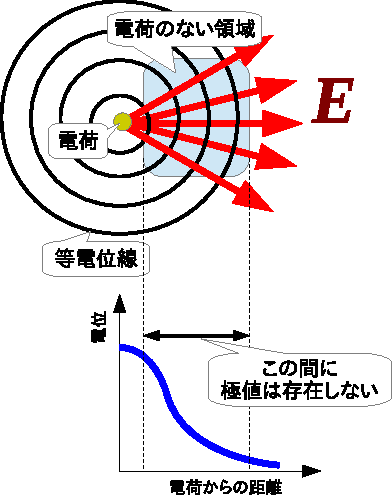
\includegraphics[keepaspectratio, width=6cm,height=7.74cm,clip]{StaticEF_Char1.pdf}
                        \caption{電荷が存在しない領域では,電位は極値をとらない}
                        \label{fig:StaticEF_Char1}
                    \end{center}
                \end{figure}

        \subsubsection{特徴2}\label{subsubsec:char2}
            等電位の閉曲面内に,電荷が存在しない場合,その内部領域全体の電位は,
            閉曲面の電位に等しく,一定である.これも,背理法で説明する.

            閉曲面の内部の電位が一定でない,と仮定する.
            閉曲面が等電位であることから,閉曲面上には電荷は存在しないので,
            この閉曲面の内側に,極値
                \footnote{
                    極値: 極大値あるは極小値のどちらかを指す総称.
                }
            が存在するはずである.
            極値が存在するということは,上記の特徴1の対偶から,
            閉曲面内に電荷が存在するはずである.
                \footnote{
                    特徴1の論理をかいつまむと,「極値が存在しない,ならば,電荷が存在しない」
                    となる.この対偶は,「電荷が存在する,ならば,極値が存在する」である.
                    一般に,「A$\Rightarrow$B」が成立するとき,その対偶「$\lnot$ B $\Rightarrow\lnot$ A」も
                    同時に成立する.
                }.
            しかし,これは,電荷が存在しないという前提に矛盾する.この矛盾は,
            閉曲面内の電位が一定でないという仮定からの帰結である.
            以上から,本特徴2を示せた.
                \begin{figure}[hbt]
                    \begin{center}
                        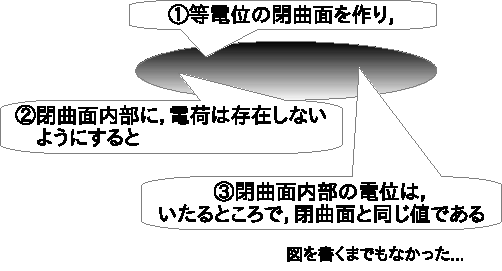
\includegraphics[keepaspectratio, width=6cm,height=5.4cm,clip]{StaticEF_Char2.pdf}
                        \caption{等電位の閉曲面内の電位(内部に電荷を含まず)}
                        \label{fig:StaticEF_Char2}
                    \end{center}
                \end{figure}


        \subsubsection{特徴3}\label{subsubsec:char3}
            任意の閉曲面において,閉曲面の内側の電荷分布と,閉曲面自体の電位が
            与えられれば,その領域内部の電位は,一意に決まる.

%       %==========================================================================
%       %  Subsection
%       %==========================================================================
        \subsection{アーンショーの定理}
        静電場中(ただし,電荷が存在しない領域に限る)では,荷電粒子は安定して存在できる
        位置がない.これを \textbf{アーンショーの定理} という
            \footnote{
                Samuel Earnshaw(1805--1888,イギリス):聖職者で数学者であった人らしい.
            }.
        この定理は,電場に限ったことではなく,磁場でも重力場でも成り立つ.
        距離に関する逆自乗の法則が成り立つならば,この定理が成立する.
                \begin{figure}[hbt]
                    \begin{center}
                        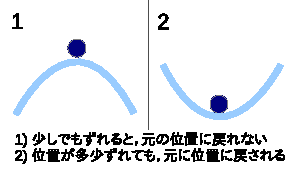
\includegraphics[keepaspectratio, width=5.11cm,height=2.91cm,clip]{Earnshow_000.pdf}
                        \caption{「安定な点」のイメージ}
                        \label{fig:Earnshow_000}
                    \end{center}
                \end{figure}

        実は,この定理は,すでに,上記の静電場の性質として,説明済みである.
        静電場に関するポアソン方程式からの帰結である.上記の性質をただ言い換えた
        だけだけど,この性質には「アーンショーの定理」とも呼ばれる別表現が
        あることを明記しておきたかった.


%   %==========================================================================
%   %  Section
%   %==========================================================================
    \section{導体}
        \begin{mycomment}
            導体といわれると,まず想像するのが,金属だろう.その他にも,
            炭素も有名だ.電解液(イオン溶液)も導体である
                \footnote{
                    ちなみに,純水は電気を通さない.水が電気を通すのは,
                    その中にイオンを含んでいる時のみであり,水道水が電気
                    を通すのも,それが完全な純水ではなく,不純物や塩素な
                    どのイオンを含んでいあるからである.
                }.
            なので,導体と言われても,想像される物質は色々と想像されてしまう.
            そこで,この章で考える導体の範囲に制限を与えることにしよう.
            ここで「導体」とよぶのは,金属や炭素などの個体で,その内部に
            自由電子をもつ物体を指すこととする.イオン溶液は確かに電気を
            通す導体ではあるが,除外する.
        \end{mycomment}

%   %==========================================================================
%   %  Subsection
%   %==========================================================================
    \subsection{導体とは}
        \subsubsection{導体,半導体,絶縁体}
        世の中には,様々な物体がある.石,木,水,葉,$\cdots$など,
        逐一例を上げていったのではきりがないほどだ.そして物体は,
        形,大きさ,硬さ,匂い,色,等,色々など性質をもっている.こういった性質の中で,
        電磁気学で特に興味がある性質に,"電気の通しやすさ" がある.
        電気の通しやすさは,物体を構成する物質そのものや,その構成に左右されるが,
        電磁気学ではそこまで細かいことは考えない
            \footnote{
                ここで学習する電磁気学は,現象論的なものである.
                物性などを含めて考えるときには,より詳細に,微視的
                な電磁気学を学習することも有用だが,内容が高度であるので,割愛する.
            }.
        目で見える範囲の物体を想像すれば十分である.
        とにかく,物体の塊を持ってきて,電気を通すか否かを判別するだけだ.
        物体の種類によって,電気の通しやすさは異なる.極端な例を上げると,
        ゴムは電気を通さないが,金属は電気を通す.様々な物体に対して,
        電気の通しやすさを調べると,それを順に並べることができる
            \footnote{
                電気の通しやすさを測定するには,対象となる物体の大きさを揃えたり,
                周囲の実験環境を揃えたりと,条件を一致させないといけない.
                ここでは,理想的に測ったと仮定しておこう.
            }.
        そうしてできた物体の順列で,電気を通しやすい部分に位置する物体のことを,
        \textbf{導体} という.反対に,電気を通しにくい部分に位置する物体のことは,
        \textbf{不導体} あるいは \textbf{絶縁体} という.
        簡単に言えば,導体とは電気を通しやすい物体のことである.
        また絶縁体は,電気を通しにくい物体のことを指す.

        ここで,"電気を通しやすい?" と表現した理由を説明しておこう
            \footnote{
                こんな回りくどい言い方をしないで,"電気を通す?" と表現したほうが,
                簡潔であると思われるかもしれないので.
            }.
        世の中には,様々な物体が存在するが,不思議な事に,「電気を(完全に)通さない
        物体」は存在しないのである.全ての物体が,電気を通すのである.ゴムなどの
        一般に電気を通さないとされる物体でも,詳細に測定すると,電気が流れることを
        確認できる.ただ,その流れる電気の量が非常に小さいので,電気を通していないと
        みなされるだけなのである.だから,電気を「通す/通さない」ではなく,
        「通しにくい/通しやすい」と書くべきなのである.

        とはいうものの,導体と絶縁体を明確に区別するような基準は存在しない.
        というか,定義すること困難なのである.導体と絶縁体とは,お互いに相対的な
        関係であり,状況によって変わりうるのである.例えば,紙は通常では絶縁体と
        して扱われるが,高電圧を紙にかける場合,電気を通すので,紙は導体として扱
        わないとならない.人間も,乾電池程度の電圧に対しては絶縁体だが,
        家庭用コンセントほどの電圧(100[V])に対しては導体となる
            \footnote{
                電化製品には,感電の恐れがあるという警告が大きく表示されているはず.
                特に,洗濯機において,アース(電気を体に通さないようにする仕組み)は絶対に
                欠かせない.
            }.
        では,導体と絶縁体の区別が全くできない程に曖昧かと
        言われれば,そうではない.\textbf{抵抗} という概念を使えば
            \footnote{
                オームの法則でお馴染みの,抵抗である.
            },
        ある程度区切りを入れることができる.抵抗による区切りも明確ではないが,抵抗は
        電気の通しやすさの1つの指標となる.
        抵抗は,電気物性を考えるときに重要な役割を果たす概念だが,電磁気学の
        理論的枠組を考える場合には,必要ではない
            \footnote{
                しかし,大切なので,後ほど解説をすることになるのだが$\cdots$.
            }.
        さしあたり,導体の例として金属をイメージすれば,十分である.また,
        絶縁体の例は,紙でも石でもゴムでもなんでもいい.
                \begin{figure}[hbt]
                    \begin{center}
                        \includegraphicslarge{DoutaiZetsuentai001.pdf}
                        \caption{導体と絶縁体}
                        \label{fig:DoutaiZetsuentai001}
                    \end{center}
                \end{figure}

        \subsubsection{理想的な導体}
            上記は,現実に存在する導体をイメージして記述した.
            これは,「物性物理学」よりの現実的な導体の説明である.
            しかし,多くの電磁気学の教科書で説明される「導体」は,
            少々異なる.
            電磁気学では,理論を考えやすくするために,理想化された導体を
            用いる.特に浸透している呼び方は無いようなので,
            このノートでは,\textbf{理想的な導体} と表現する.
            理想的な導体が,現実の導体と違う点を,いくつか上げておこう
                \footnote{
                    全部を上げることはできない.というか,思いつく限り上げたところで,
                    それで十分かどうかを判断することができないから.いや,
                    「理想的な導体」を理論的に整合性を保つように定義してやれば,
                    可能なのだけど,興味がない
                    (そんなことに時間をかけたくない,ってのが本音).
                }.
            \begin{myshadebox}{理想的な導体の性質}
                理想的な導体が持つ性質は,次の通り.
                \begin{enumerate}
                    \item 電荷には大きさがない(これは電磁気学全体をとおして同じ)
                    \item 正電荷と負電荷は導体中を自由に移動できる
                    \item 無限に多くの電荷をもっている(電荷の数に上限を与えない)
                    \item 導体中の電荷は,導体の外に出ることはできない
                    \item 連続分布している(原子レベルの不連続状態は考えない)
                \end{enumerate}
            \end{myshadebox}

            考えればいくらでも出てきそうだ
                \footnote{
                    教科書には,大抵の場合,こういった
                    ことは暗黙の了解として,明記されていない.紙面がもったいないからだろうか.
                    まあ,こんな約束なら,読めば簡単に悟れるから書くまでもないか.
                    書き始めるとキリがないし.
                }.
            この辺りで列挙を止めておこう.あとは,気が向いたら追記することにして,
            話をすめよう.

            上記の箇条書きに対して,補足しておきたい.理想的な導体を考える場合,
            それは原子で構成されていると考えてはいけない.確かに,正電荷と負電荷
            を持っているが,正電荷も導体内を自由に移動できるからだ.現実には,
            導体は原子で構成されていて,正電荷は動けない.正電荷も導体内を自由に移動
            できるという点が,はじめは違和感を感じるかもしれない.
                \begin{figure}[hbt]
                    \begin{center}
                        \includegraphicsdefault{risouteki_na_doutai000.pdf}
                        \caption{理想的な導体のイメージ}
                        \label{fig:DoutaiZetsuentai001}
                    \end{center}
                \end{figure}


%   %==========================================================================
%   %  Subsection
%   %==========================================================================
    \subsection{導体と電場の関係}
        \subsubsection{静電誘導}
        電場には,面白い性質がある.導体で囲まれた空間内部には電場は存在不可能
        なのである.導体はその内部に自由電子を含んでいる.この自由電子が,
        導体の外側の電場を打ち消すのである.
        自由電子は,導体中で移動できるため,導体の外側の電場から,
        クーロン力を受ける.自由電子は導体中に多数存在し,
        クーロン力に釣り合うように分布し,静止する.
        こうして静止した自由電子は,導体の外側の電場を完全に打ち消すように
        分布する.

        導体内部の自由電子が,外側の電場によって園分布が変わる現象を,
        \textbf{静電誘導} という.電子が電場に誘導されるイメージ.

        さらに言うと,電場は導体の表面で吸収され,導体中には浸透しない.
        導体内部が空洞だろうとなかろうと,導体の内部では一切電場は発生しない.
                \begin{figure}[hbt]
                    \begin{center}
                        \includegraphicsdefault{Doutai_to_Denba001.pdf}
                        \caption{静電誘導}
                        \label{fig:Doutai_to_Denba001}
                    \end{center}
                \end{figure}


        もちろん,電場を与えた
            \footnote{
                あるいは,電場の状態を変更しても同じこと.
            }
        直後は電荷の移動が起こるため,この間,導体内部にも電場が生じている.
        電荷がどのようにして導体中を移動するかも,興味のあるところだけど,
        ここでは,静電場内の現象を考えたいので,電荷の移動のことは後回し
        にしておこう.ここで考えたいことは,電荷の移動が完了したの,
        導体周辺に生じる静電場である.

        \subsubsection{静電遮蔽}
        上記の静電誘導の見方を変えると,
        導体の内部まで電場が突き抜けることはない,と言っても同じことだ.
        こうした立場からは,この現象を \textbf{静電遮蔽} という
            \footnote{
                あるいは,\textbf{静電シールド} とよばれれることもある.
            }.
        導体が電場を遮蔽するのだ.
                \begin{figure}[hbt]
                    \begin{center}
                        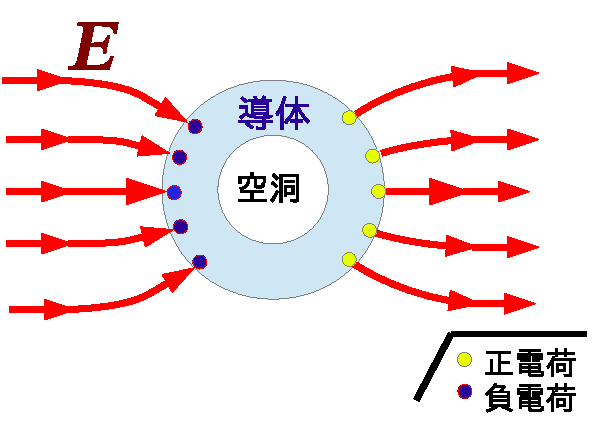
\includegraphics[keepaspectratio, width=6cm,height=4.2cm,clip]{Doutai_to_Denba000.pdf}
                        \caption{静電遮蔽}
                        \label{fig:Doutai_to_Denba000}
                    \end{center}
                \end{figure}

        電場の影響を極力少なくした実験を行う場合,この静電遮蔽が有効である.
        導体に完全に囲まれていれば,その中には電場は侵入してこないのだ.

        \begin{memo}{導体内部に電場は生じない}
            背理法を使って説明しよう(エネルギー保存則との矛盾をつかう).
            もし導体中に電場が発生すると仮定する.
            この時,導体内部の自由電子が,静電誘導を受け移動が始まる.
            しかし,これはエネルギー保存則に反する.なぜなら,
            エネルギーを与えていないにもかかわらず(電場はエネルギーではない),
            電流が生じるはずがないからだ.

            というか,そもそも,導体である条件の1つに,数え切らないくらいの
            自由電子をもっているという性質が要請されていて,電子は電場を吸収する
            のであるから,導体内部に電場が発生しないことは,導体の定義から直接的に
            示されるとも考えられる.
        \end{memo}

        \subsubsection{電場と導体表面}
        電場が導体の表面で吸収される場合,電場は導体表面に直交する.
        導体の形状がどんなに複雑でも,電場は表面に直角に交わる.
                \begin{figure}[hbt]
                    \begin{center}
                        \includegraphicsdefault{Doutai_to_Denba002.pdf}
                        \caption{電場は導体表面に直交する}
                        \label{fig:Doutai_to_Denba002}
                    \end{center}
                \end{figure}

        斜めに交わることはない.もし,斜めに交わってしまうと,導体表面に平行な電場成分が発生する.
        しかし,これは,先に示した導体の性質「導体内部に電場は生じない」と反する.だから,
        道内の内部に電場が生じないように交わるには,直角に交わるしかないのだ.
                \begin{figure}[hbt]
                    \begin{center}
                        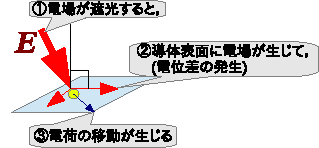
\includegraphics[keepaspectratio, width=6cm,height=2.7cm,clip]{Doutai_to_Denba003.pdf}
                        \caption{もし,電場が導体に直交しなかったら...}
                        \label{fig:Doutai_to_Denba003}
                    \end{center}
                \end{figure}

%   %==========================================================================
%   %  Subsection
%   %==========================================================================
    \subsection{導体と電位の関係}
    導体の表面は等電位面である.導体がどんな形をしていても,等電位面になる.
    電場が導体に垂直に交わることから,簡単に説明できる.
    \ref{subsec:toudeni_denba}節を参照.


